vanier%Background body
%Created MS 05-11

\section{Background}\label{background}

\subsection{Optical Pumping}\label{opticalpumping}

Optical pumping is the process in which the interaction of light with
atoms produces a population of energy levels that is distinct from the
thermal equilibrium Boltzmann distribution \cite{bernheim}. In a
three-state system, with a ground state $|g\rangle$, excited state
$|e\rangle$, and intermediate metastable state $|m\rangle$
(Fig. \ref{pumping}), it is possible to selective populate the metastable
state if the natural decay time $\gamma_{rel}$ is sufficiently long in
comparison to the pumping time. If laser light is applied on resonance
with the $|e\rangle$ to $|g\rangle$ transition, it drives the atom
population to the excited state, and then the atoms decay to the lower
energy levels with some time constant. If the laser light cannot
excite atoms from the metastable state to the excited state (for
example, due to selection rules), the process preferentially populates
the state $|m\rangle$, resulting in optical pumping.


\begin{figure}[h]
\begin{center}
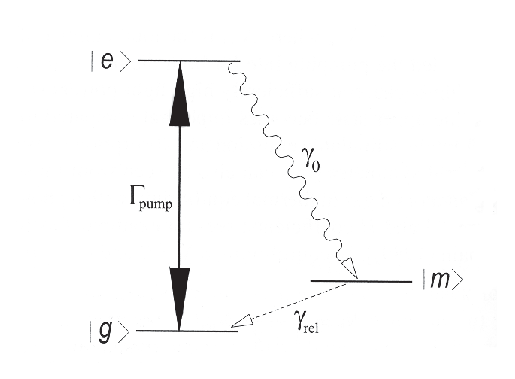
\includegraphics[width=4in]{figures/pumping.eps}
\caption{\small{Three level system with optical pumping rate $\Gamma_{pump}$}}
\label{fig:pumping}
\end{center}
\end{figure}


\subsection{Rubidium System}

In this experiment, we consider an ensemble of rubidium atoms as an
optical pumping system. Rubidium is an alkali atom with a single
electron in its outer shell, and thus can be modelled as a
hydrogen-like system. Here, we take the outer $5^2S_{1/2}$ level as
the ground state and focus on the $D_1$ transition between the
$5^2S_{1/2}$ and $5^2P_{1/2}$ states. 

We use a natural abundance Rubidium cell for optical pumping, which
consists of $72\%$ $^{85}$Rb and $28\%$ $^{87}$Rb, so we are able to
investigate the properties of both isotopes. The energy level diagrams
are presented in Fig.~\ref{fig:8587levels}.


\begin{figure}[h]
\begin{center}
\subfigure[$^{87}$Rb energy spectrum]{\label{fig:edge-b}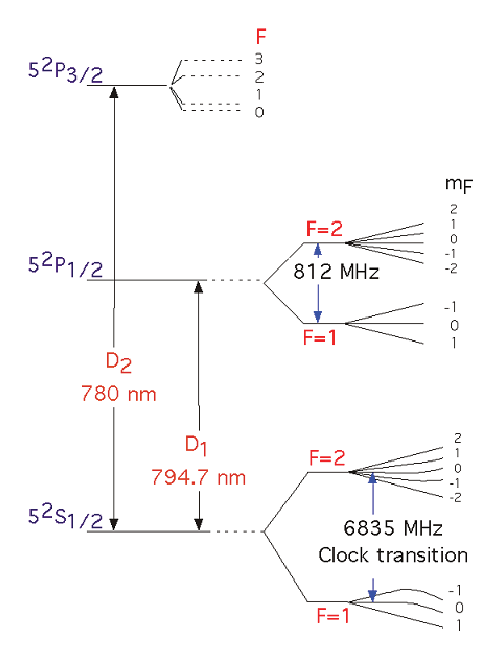
\includegraphics[height=3.5in]{figures/87levels.eps}}
\hspace{-1mm}
\vspace{-2mm}
\subfigure[$^{85}$Rb energy spectrum]{\label{fig:edge-a}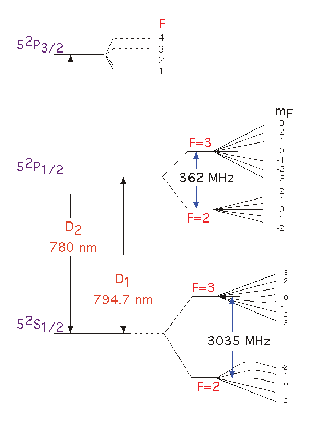
\includegraphics[height=3.5in]{figures/85levels.eps}}
\vspace{-2mm}
\caption{\small{CAPTION GOES HERE}}
\label{fig:8587levels}
\end{center}
\end{figure}

There are several levels of splitting which occur in the Rb atom. The
splitting of the $5^2P$ state into $5^2P_{1/2}$ and $5^2P_{3/2}$ is
due to spin-orbit coupling, that is, the addition of the spin and
orbital angular momenta ($S$ and $L$, respectively) of the electrion
to comprise the total angular momentum $J$. As mentioned above, the
laser has been tuned to the $D_1$ line because of its better optical
pumping properties (Fig.~\ref{fig:8587levels}).

In addition, each total electron angular momentum level is further
split by the coupling of spins of the electron to the nucleus, known
as hyperfine splitting. This results in the distinct $F$ levels, where
$F = I + J$; $I$ is the spin of the nucleus and $J$ as above is the
total electron angluar momentum. Each pair of $F$ states in these
levels of Rb is separated by a frequency shift on the order of
hundreds or thousands of MHz, allowing the tuning of the laser to a
particular transition (Fig.~\ref{fig:fluor}). For instance, we
chose to focus on the $^{85}$Rb $5^2S_{1/2}, F = 3$ to $5^2P_{1/2}, F
= 3$ transition for most of the experiment, because the density of the
$^{85}$Rb isotope is over twice as high, and the $3$ to $3$ line is
more easily separated from the neighboring transitions.

\begin{figure}[h]
\begin{center}
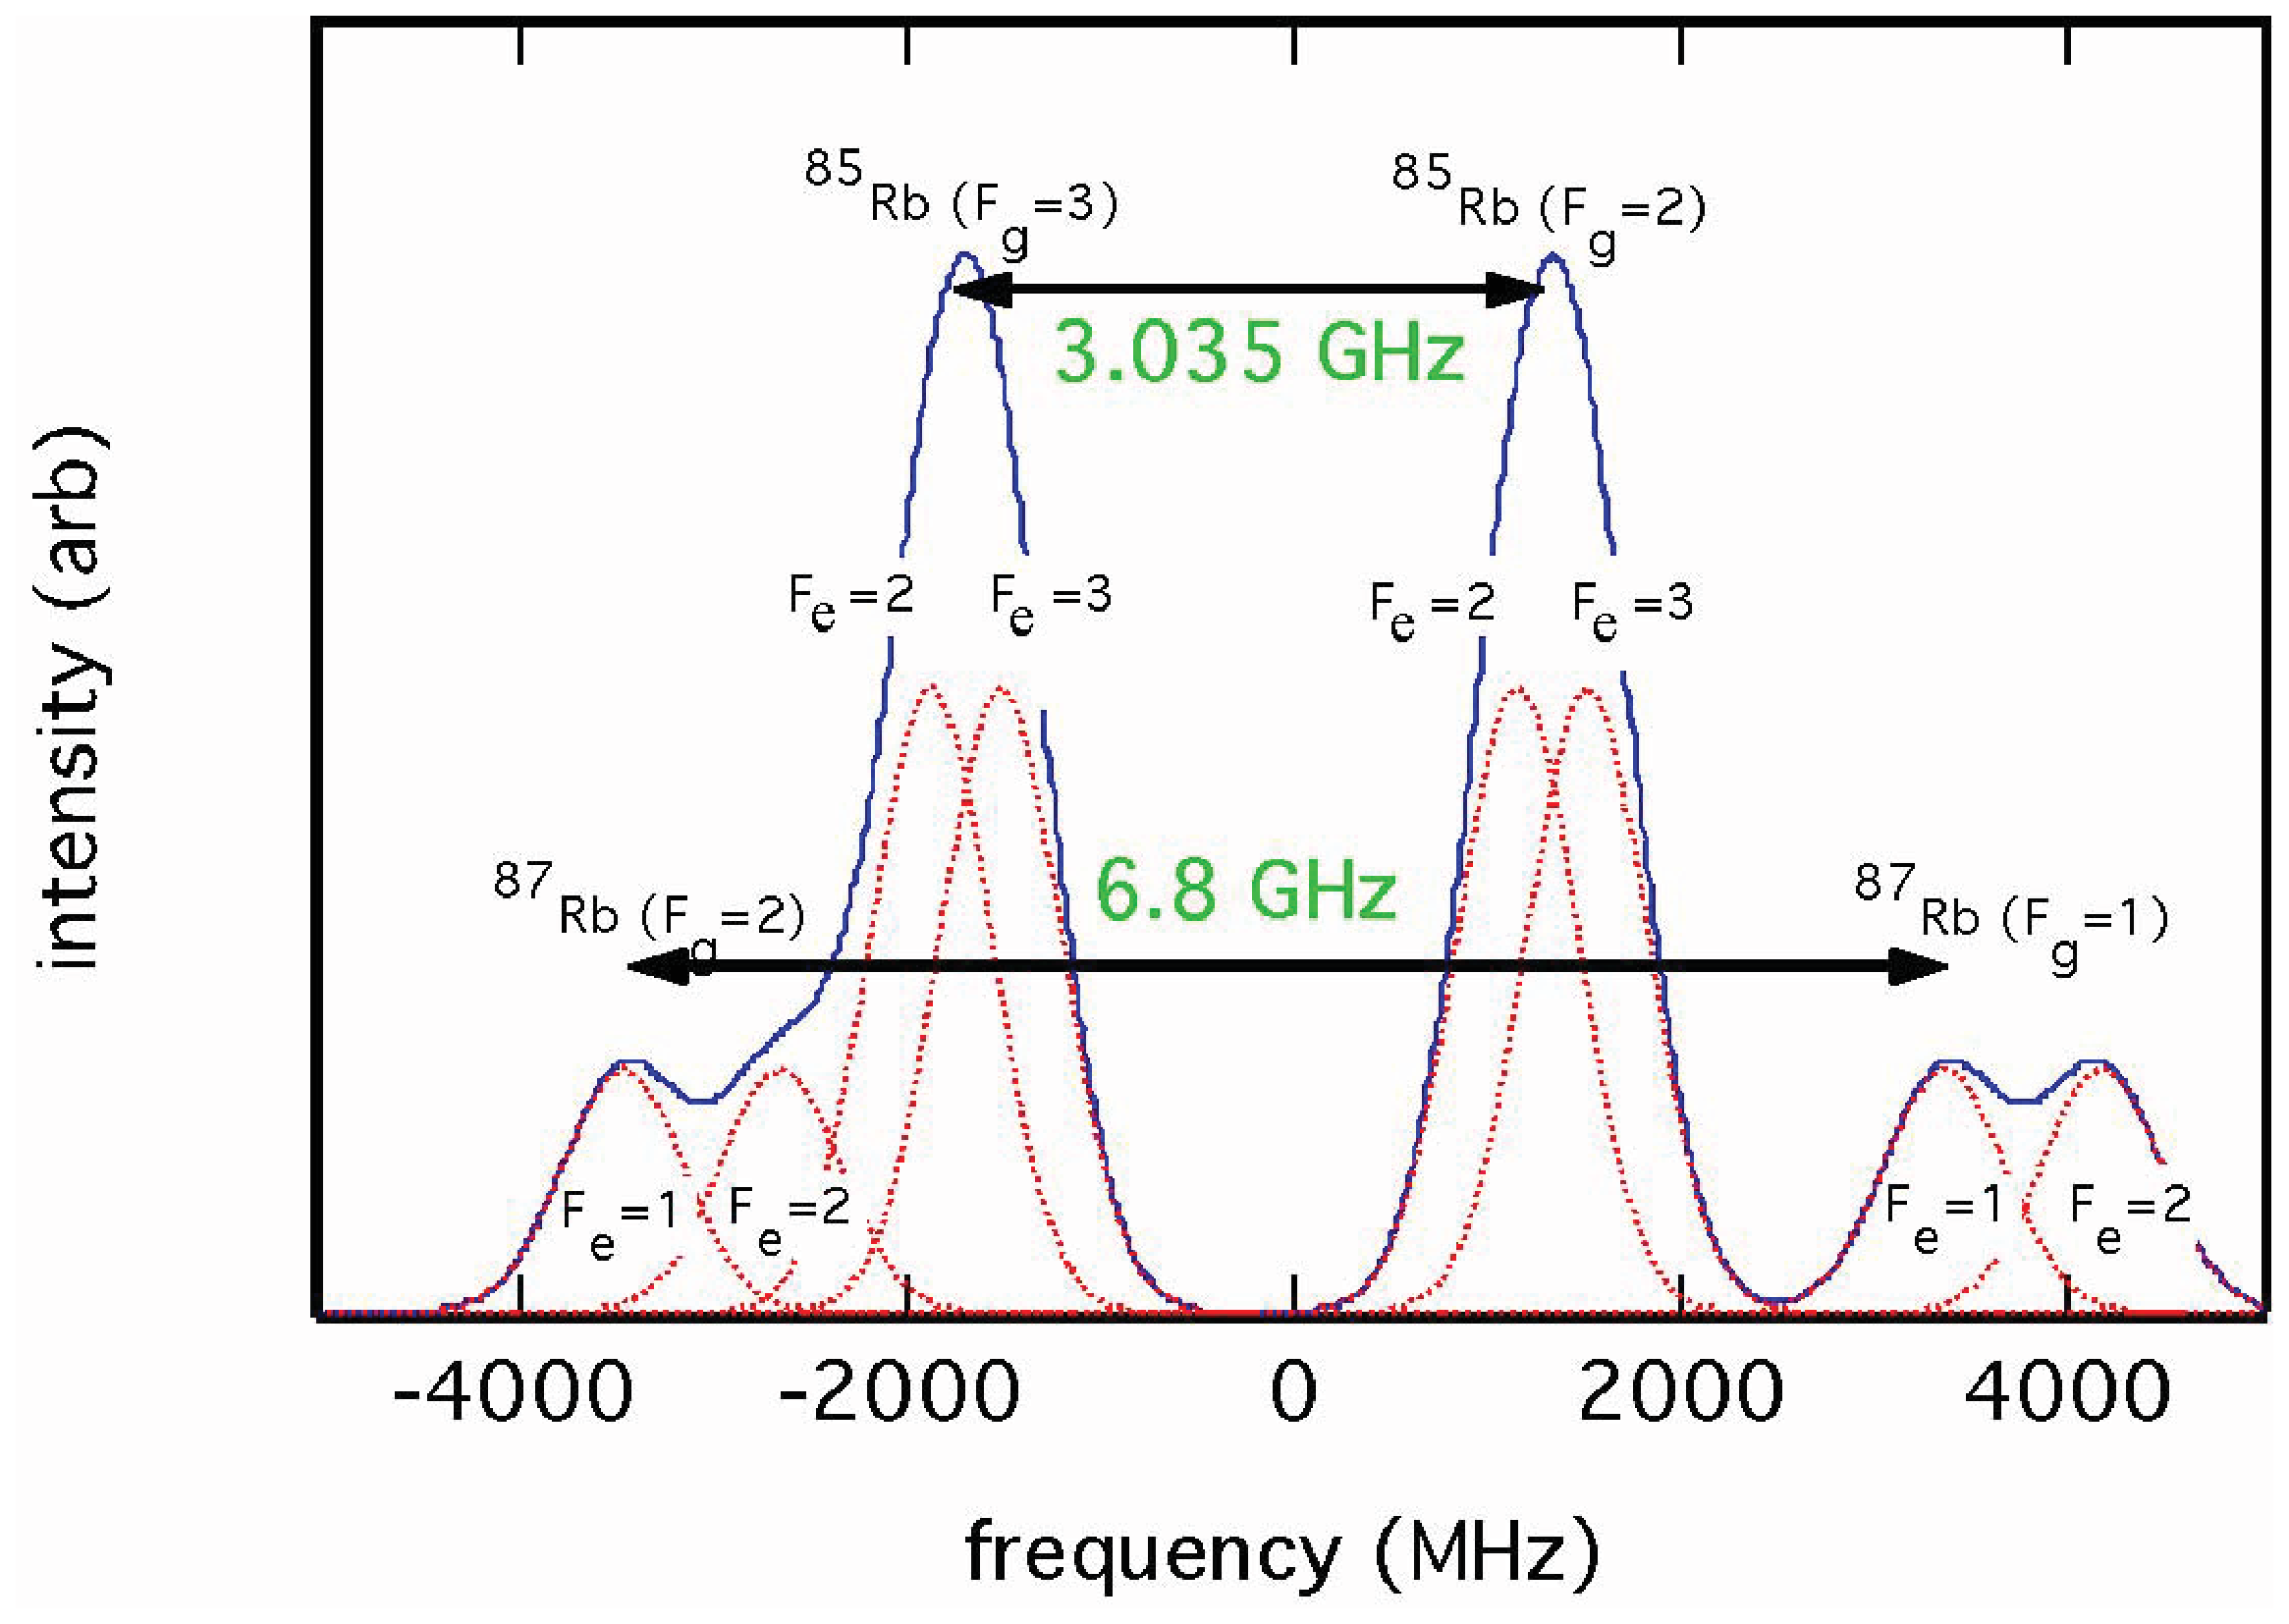
\includegraphics[height=3in]{figures/fluorescence.eps}
\caption{\small{Fluoresence spectrum of natural abundance rubidium. The $x$-axis is a relative measure of frequecy, with $0$ being the $D_1$ transition frequency. The dashed red line represents the fluorescence from individual transitions, and the blue line is the combined intensity.}}
\label{fig:fluor}
\end{center}
\end{figure}

Further splitting occurs in the Zeeman effect, where the degenerate
magnetic sublevels are split via an application of a uniform magnetic
field. For weak fields, the splitting is directly proportional to $B$,
the magnetic field amplitude and the magnetic dipole moment. The
change in the energy is given by

\begin{equation}
\Delta E = g_F\mu_B B m_F
\label{eqn:zeeman}
\end{equation}

where $\mu_B = \frac{e\hbar}{2m_e}$ is the Bohr magneton, $B$ is the
$z$-projection of the magnetic field, and $m_F$ is the spin projection
in the $z$ direction of the total angluar momentum of the atom
\cite{budker }. The qualitative dependence of these splittings on
magnetic field amplitude can be seen in Fig.~\ref{fig:8587levels},
where the energy split between initally degenerate levels increases
with magnetic field.

In our experiment, the different splittings of the rubidium levels are
used as an effective 3-level system, as described in
section\ref{opticalpumping}. Although there are many levels in a
rubidium atom, it is valid to approximate the system as composed of
only the $5^2S_{1/2}$ and $5^2P_{1/2}$ sublevels if the laser is on
the $D_1$ line, and does not interact with the states which are not on
resonance. We treat the set of $5^2S_{1/2}$ levels as the ground
states, and $5^2S_{1/2}$ as the excited states. 

By applying a uniform magnetic field, the magnetic sublevels are
split, and one can act as the metastable ``dark''state $|m\rangle$
necessary for optical pumping as follows: if $\sigma_+$-polarized
laser light is applied to the atom, then the only allowed transitions
to an excited state are those with $\Delta m_F = +1$.
(Fig.~\ref{fig:rbpump}). In the case of a $F = 1$ to $F = 1$
transition, for instance, the ground state with $m_F = 1$ is the
`dark' state because it cannot absorb $\sigma_+$ light. However, atoms
do get excited from the $m_F = -1, 0$ states, and then spontaneously
decay into all three ground states. Therefore, there is an overall
positive rate of atoms going into the `dark' state, increasing
transmission and creating the conditions of optical pumping, as desired. 

\begin{figure}[h]
\begin{center}
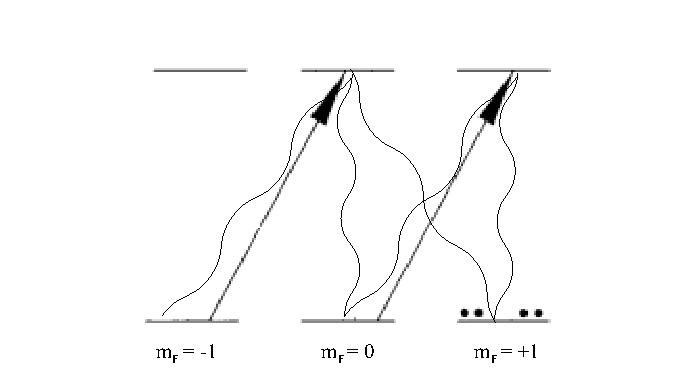
\includegraphics[height=2.5in]{figures/rbpump.eps}
\caption{\small{Effects of optical pumping on the $1\rightarrow 1$
    transition with $\sigma_+$ light on the populations of the ground
    state Zeeman levels. Due to quantum exclusion rules, the ground
    $m_F = +1$ state is `dark' to the laser, and so atoms get
    preferentially pumped into this state.q}}
\label{fig:fluor}
\end{center}
\end{figure}


\subsection{Magnetic Interactions}

In order to study the properties of the rubidium atoms, such as the
g-factor, we introduce a magnetic field transverse to the $z$
direction established by the laser and uniform magnetic field. This
field is introduced at a RF on the order of the Zeeman splittings,
coupling the dark state with the ground states. 

\subsubsection{Rabi Oscillations}

For a two-level system with ground state energy $E_2$ and excited
state energy $E_1$, the application of a periodic perturbation of the
form $V(t) = V_0e^{i\omega t}$ with a relaxation (damping) term
proportional to a constant $\Gamma$, the time dependence of the
population of the upper state is given by

\begin{equation}
P(t) = \frac{(2V_0)^2e^{-\Gamma t/2}}{(2V_0)^2 +\Delta^2 + \Gamma^2/4}\sin^2(\frac{t}{2}\sqrt{(\Delta + \Gamma/2)^2 + (2V_0)^2})
\end{equation}

Here, $\Delta = \omega - \omega_0$ is the detuning, with $\omega_0 =
(E_1 - E_2)/\hbar$ the separation between the upper and lower state of
the system, and $\omega$ the frequency of the periodic
perturbation. $\Gamma$ is the natural decay rate of the population in
the excited state \cite{budker}.

This gives the general behavior of a driven, damped optical system. In
the case of a three level system, it is useful to make the
approximation of a small RF perturbation on top of the pumping
system. in that case the logic of the above discussion applies


\subsection{Rate Equations}\label{rateequations}

\subsubsection{Power Broadening}

\subsubsection{Time Constants}

$\tau$ is the optical pumping time, which is the time it takes to
change the total magnetization from thermal equilibrium to the maximal
equilibrium value with the presence of an external electromagnetic
field.

$T_1 = 1/\gamma_1$ is time constant of longitudinal relaxation,
i.e. the time that the diagonal elements of the density matrix
$\rho_{jj}$ return to the equilibrium in the absence of other
perturbations \cite{vanier} p79.

\begin{equation}
\gamma_1 = \gamma_1^{se} + \gamma_1^{w} + \gamma_1^{bg} 
\label{eqn:gamma1}
\end{equation}

where $\gamma_1^{se}$ is the spin exchange rate, $\gamma_1^{w}$ is the
wall collision rate due to leaving the beam, and $\gamma_1^{bg}$ is
the rate due to buffer gas collisions \cite{vanier}.

$\gamma_2$ is the coherence relaxation rate; the off-diagonal elements
$\rho_{ij}$:

\begin{equation}\gamma_2 = \gamma_2^{se} + \gamma_2^{w} + \gamma_2^{bg}
\label{eqn:gamma2}
\end{equation} 

\subsection{Spin Exchange}


Spin exchange is the ability of two particles to transfer their spin
orientation to one another upon making a collision (needs to be
paraphrased) \cite{bernheim}. Let $A$ and $B$ be two $^2S_{1/2}$
alkali atoms. Then a spin-exchange collision between the two atoms
can be represented by the equation

\begin{equation}
A(\uparrow) + B(\downarrow) \rightarrow A(\downarrow) + B(\uparrow)
\end{equation}

so the spin orientations of the two atoms are exchanged, while the
total spin is conserved \cite{happer}.  

The mechanism of spin exchange is one of the largest factors
contributing to the natural linewidth of the RF resonance ($T_2$ time) and
the $T_1$ time \cite{vanier}. In addition, spin exchange is a valuable
technique of studying the properties of an atom or particle for which
a direct optical particle procedure is much more difficult.

In this experiment, we use the spin exchange mechanisms between
$^{85}$Rb and $^{87}$Rb in order to study the contribution of spin
exchange collisions to the inherent RF linewidth of the two isotopes
(Eqn.~\ref{eqn:gamma2}).

\subsection{Inhomogeneous Broadening}

In Section~\ref{rateequations} above, the homogeneous broadening
mechanisms contributing to the line width of $\gamma_2$ and
$\gamma_1$. In the case of homogeneous broadening, the assumption is
made that the interaction of the electromagnetic fields with the
individual magnetic moments of the atoms that has the same features
for every member of the atomic ensemble. In this case, every sample of
atoms is representative of the average behaviour of the entire system
\cite{vanier}. 

In the case of inhomogeneities in the system, further broadening can
occur. The most common causes of inhomogeneous broadening relevant to
our optical pumping experiment are Doppler effects and magnetic field
inhomogeneities. The additional broadening $\nu_D$ due to the Doppler effect
is given by

\begin{equation}
\nu_D = 2\nu_0\sqrt{\frac{2 k T}{M c^2}\ln{2}}
\end{equation}

where $\nu_0$ is the unbroadened linewidth, $k$ is Boltzmann's
constant, $T$ is temperature of the gas and $M$ is the atomic mass of
the gas \cite{yariv}. For the quantities in our experiment, the
Doppler linewidth addition is $6$ orders of magnitudes smaller than
the natural width, so it is not a detectable effect for the present
conditions.

The effect of magnetic field inhomogeneity is much more difficult to
express analytically, because it depends on the nature of the
inhomogeneities. Generally, the overall line shape can be expressed as
a sum of individual homogeneously broaded lines, $i.e.$ Lorentzians,
with a range of cneter frequencies
(Fig~\ref{inhomo})\cite{vanier}. The broadening occurs because
different samples of atoms will effectively experience different
amplitudes of the magnetic field due to the inhomogeneity, thus
resulting in a range of Zeeman splittings and a range of center
frequencies for the ensemble's resonance.

\begin{figure}[h]
\begin{center}
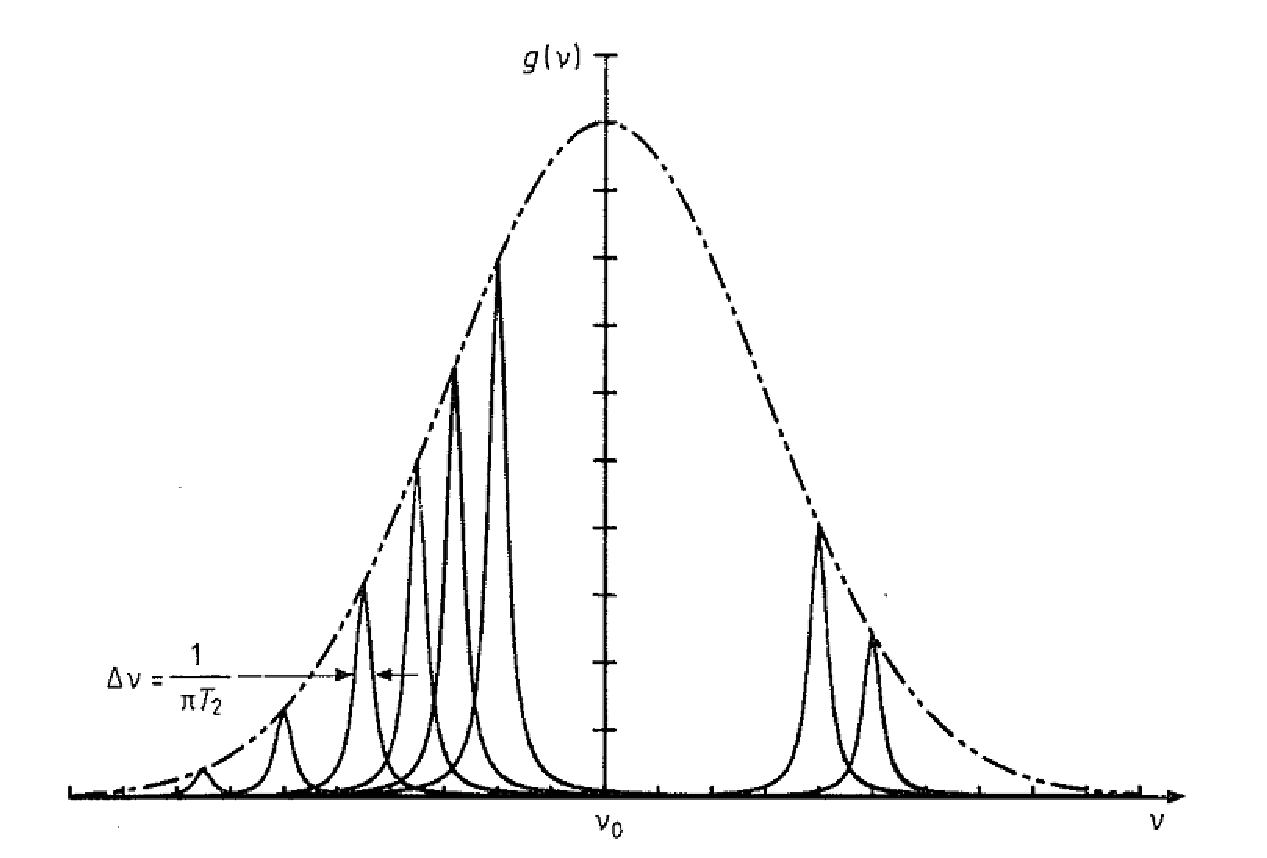
\includegraphics[height=3in]{figures/inhomogeneous.eps}
\caption{\small{In the event of inhomogeneities in the system ($e.g.$ in the uniform magnetic field), the overall linewidth of the RF resonance becomes broadened. The general form of the broadening is shown above, where each portion of the population of atoms is experiences a different B field amplitude and has a different center frequency.}}
\label{fig:inhomo}
\end{center}
\end{figure}


